\documentclass[svgnames,
               hyperref={colorlinks,citecolor=DeepPink4,linkcolor=FireBrick,urlcolor=Maroon},
               usepdftitle=false]  % see \hypersetup{} below
               {beamer}

\mode<presentation>{
  \usetheme{Madrid}
  %\usecolortheme{seagull}
  \usecolortheme{seagull}
  \setbeamercovered{transparent}
  \setbeamerfont{frametitle}{size=\large}
}

\setbeamercolor*{block title}{bg=red!10}
\setbeamercolor*{block body}{bg=red!5}

%\usepackage[svgnames]{xcolor}
\usepackage{hyperref}
\hypersetup{
    pdftitle = {A full approximation scheme multilevel method for solving nonlinear variational inequalities},
    pdfauthor = {Ed Bueler and Patrick Farrell},
    pdfsubject = {},
    pdfkeywords = {}
}

\usepackage[english]{babel}
\usepackage[latin1]{inputenc}
\usepackage{times}
\usepackage[T1]{fontenc}
\usepackage{empheq,bm,xspace,fancyvrb,soul}
\usepackage{tikz}
\usetikzlibrary{shapes,arrows.meta,decorations.markings,decorations.pathreplacing,fadings,positioning}
\usepackage[kw]{pseudo}
\pseudoset{left-margin=15mm,topsep=5mm,label=,idfont=\texttt,st-left=,st-right=}

\makeatletter
%\newcommand\notsotiny{\@setfontsize\notsotiny\@vipt\@viipt}
\newcommand\notsotiny{\@setfontsize\notsotiny\@viipt\@viiipt}
\makeatother

\newcommand{\eps}{\epsilon}
\newcommand{\RR}{\mathbb{R}}

\newcommand{\grad}{\nabla}
\newcommand{\Div}{\nabla\cdot}
\newcommand{\trace}{\operatorname{tr}}

\newcommand{\hbn}{\hat{\mathbf{n}}}

\newcommand{\bb}{\mathbf{b}}
\newcommand{\be}{\mathbf{e}}
\newcommand{\bbf}{\mathbf{f}}
\newcommand{\bg}{\mathbf{g}}
\newcommand{\bn}{\mathbf{n}}
\newcommand{\bq}{\mathbf{q}}
\newcommand{\br}{\mathbf{r}}
\newcommand{\bu}{\mathbf{u}}
\newcommand{\bv}{\mathbf{v}}
\newcommand{\bw}{\mathbf{w}}
\newcommand{\bx}{\mathbf{x}}

\newcommand{\bF}{\mathbf{F}}
\newcommand{\bQ}{\mathbf{Q}}
\newcommand{\bU}{\mathbf{U}}
\newcommand{\bV}{\mathbf{V}}
\newcommand{\bX}{\mathbf{X}}

\newcommand{\btau}{\bm{\tau}}
\newcommand{\bxi}{\bm{\xi}}

\newcommand{\bzero}{\bm{0}}

\newcommand{\cK}{\mathcal{K}}
\newcommand{\cV}{\mathcal{V}}

\newcommand{\rhoi}{\rho_{\text{i}}}

\newcommand{\ip}[2]{\left<#1,#2\right>}

\newcommand{\nn}{{\text{n}}}
\newcommand{\pp}{{\text{p}}}
\newcommand{\qq}{{\text{q}}}
\newcommand{\rr}{{\text{r}}}

\newcommand{\ds}{\displaystyle}

\newcommand{\bus}{\bu|_s}
\newcommand{\oo}[1]{\displaystyle O\left(#1\right)}
\newcommand{\sold}{s_{\text{o}}}

\newcommand{\maxR}{R^{\bm{\oplus}}}
\newcommand{\minR}{R^{\bm{\ominus}}}
\newcommand{\iR}{R^{\bullet}}

\newcommand{\sdoi}[1]{\,{\tiny \href{https://doi.org/#1}{doi:#1}}}



\title[FASCD = multigrid for VIs]{A full approximation scheme multilevel method \\ for solving nonlinear variational inequalities}

%\subtitle{\emph{}}

\author[Bueler and Farrell]{Ed Bueler \inst{1} \and Patrick Farrell \inst{2}}
\institute[]{\inst{1} University of Alaska Fairbanks \and %
             \inst{2} Mathematical Institute, Oxford University}

\date[]{ISMP 2024}

%\titlegraphic{\begin{picture}(0,0)
%    \put(0,180){\makebox(0,0)[rt]{\includegraphics[width=4cm]{figs/software.png}}}
%  \end{picture}
%}

\titlegraphic{\vspace{-18mm} 
\includegraphics[width=0.2\textwidth]{../talk-oxford/images/uafbw.png} \hfill \begin{minipage}{0.12\textwidth}

\includegraphics[width=\textwidth]{../talk-oxford/images/oxford.png}

\vspace{18mm}
\end{minipage} \vspace{-10mm}}

%% to start section counter at 0 see
%% https://tex.stackexchange.com/questions/170222/change-the-numbering-in-beamers-table-of-content


\begin{document}
\beamertemplatenavigationsymbolsempty

{
  %\usebackgroundtemplate{\includegraphics[width=\paperwidth]{../talk-oxford/images/gray-british-clark2022.png}}
  \begin{frame}

\vspace{10mm}

    \titlepage
  \end{frame}
}


\begin{frame}{Outline}
  \tableofcontents

\only<1>{\phantom{\emph{warning:} no convergence theorem}}
\only<2>{\emph{warning:} no convergence theorem}
\end{frame}


\section{variational inequalities (VIs)}

\begin{frame}{{\color{FireBrick} variational inequality} $=$ constrained weak form equations}

\begin{center}
\begin{tabular}{r|l|l}
& \qquad unconstrained & \qquad constrained \\ \hline
optimization &
\begin{minipage}[t][16mm][t]{0.32\textwidth}
$$\min_{u\in\mathcal{V}} J(u)$$
\end{minipage}
&
\begin{minipage}[t][16mm][t]{0.35\textwidth}
$$\min_{u\in\mathcal{K}} J(u)$$
\end{minipage}
\\ \hline
\only<1>{equations}\only<2->{\begin{minipage}[t][16mm][t]{0.15\textwidth} weak form \par equations \end{minipage}} &
\begin{minipage}[t][16mm][t]{0.32\textwidth}

\vspace{-2mm}
find $u \in \mathcal{V}$:
\only<1>{$$F(u)=0$$}
\only<2->{$$\ip{F(u)}{v} = 0 \quad \forall v \in \mathcal{V}$$}
\end{minipage}
&
\begin{minipage}[t][16mm][t]{0.35\textwidth}

\vspace{-2mm}
\only<3>{
{\color{FireBrick} find $u \in \mathcal{K}$:}
$${\color{FireBrick} \ip{F(u)}{v-u} \ge 0 \quad \forall v \in \mathcal{K}}$$
}
\end{minipage}
\end{tabular}
\end{center}

\bigskip

\begin{itemize}
\item where $\mathcal{K} \subset \mathcal{V}$ is closed and convex
\item<3> sometimes the {\color{FireBrick} variational inequality (VI)} is the KKT condition of optimization ($F=J'$), and sometimes not
\end{itemize}
\end{frame}


\begin{frame}{example: classical obstacle problem}

\begin{center}
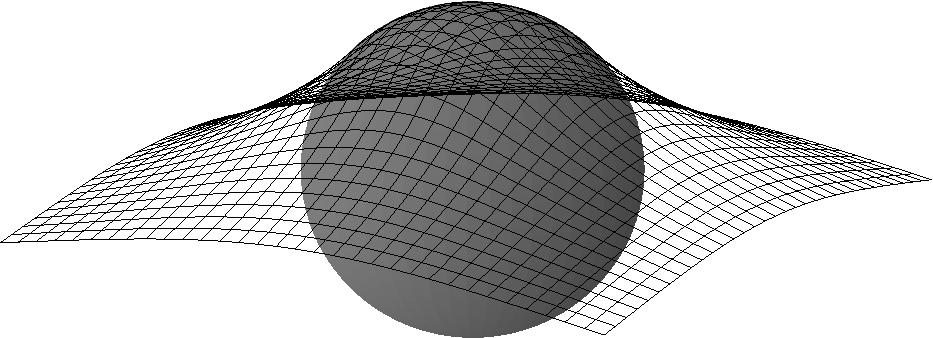
\includegraphics[width=0.65\textwidth]{../talk-oxford/images/obstacle65.pdf}
\end{center}

\begin{itemize}
\item \emph{problem.} on $\Omega \subset \RR^2$, find $u(x)$ which minimizes
    $$J(v) = \int_\Omega \frac{1}{2} |\grad v|^2 - f\, v$$
over
    $$\mathcal{K} = \left\{v \in H^1(\Omega) \,:\, v\big|_{\partial \Omega} = g \,\text{ and }\, v \ge \psi\right\}$$
\end{itemize}
\end{frame}


\begin{frame}{example \dots and VI language}

\begin{minipage}[t]{0.55\textwidth}
\vspace{0pt}
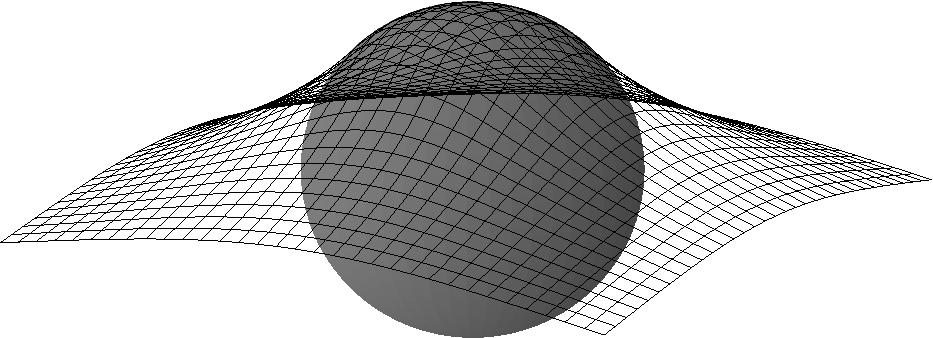
\includegraphics[width=\textwidth]{../talk-oxford/images/obstacle65.pdf}
\end{minipage}
\hfill
\begin{minipage}[t]{0.3\textwidth}
\vspace{2mm}
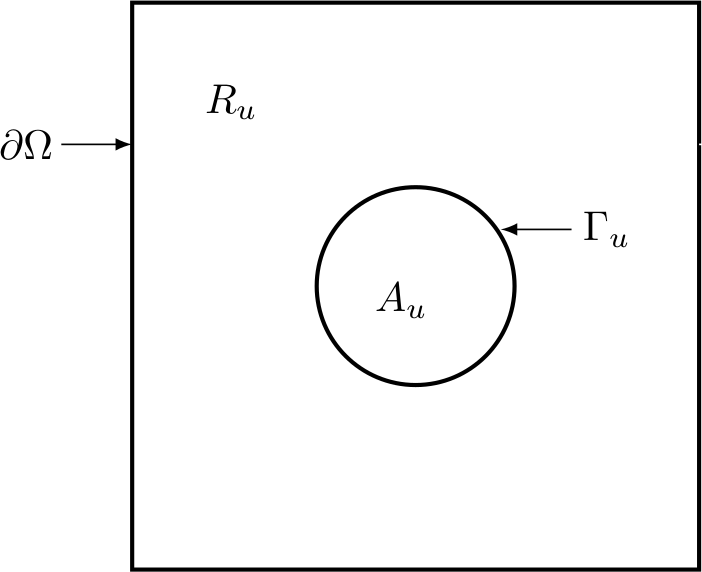
\includegraphics[width=\textwidth]{../talk-oxford/images/obstacle-sets.png}
\end{minipage}

\vspace{-1mm}
\begin{itemize}
\item the solution defines subsets of $\Omega$:
   \begin{itemize}
   \item[$\circ$] \emph{active set} \quad $A_u = \{u = \psi\}$
   \item[$\circ$] \emph{inactive set} \quad $R_u = \{u> \psi\}$
   \item[$\circ$] \emph{free boundary} \quad $\Gamma_u=\partial R_u \cap \Omega$
   \end{itemize}
\item the \emph{complementarity problem} (CP) is a PDE-like strong form:
\begin{equation*}
u - \psi \ge 0, \qquad -\grad^2 u - f \ge 0, \qquad (u - \psi)(-\grad^2 u - f) = 0
\end{equation*}
\item the weak form is the VI:
    $$\int_\Omega \grad u\cdot \grad (v-u) - f (v-u) \ge 0 \quad \forall v \in \mathcal{K}$$
\end{itemize}
\end{frame}


\begin{frame}{variational inequalities: general setting}

\begin{itemize}
\item $\mathcal{K}$ is a closed and convex subset of a Banach space $\mathcal{V}$
\item $F:\mathcal{K} \to \mathcal{V}'$ is a continuous operator
    \begin{itemize}
    \item[$\circ$] $F$ is generally nonlinear
    \item[$\circ$] $F$ may be defined \emph{only} on $\mathcal{K}$
    \item[$\circ$] $F$ may \emph{not}\, be the derivative of an objective function $J$
    \end{itemize}
\item the variational inequality {\color{FireBrick} VI($F$,$\mathcal{K}$)} is to find $u\in\cK$ so that
	$${\color{FireBrick} \ip{F(u)}{v-u} \ge 0 \quad \text{ for all } v \in \mathcal{K}}$$

    \begin{itemize}
    \item[$\circ$] for nontrivial $\mathcal{K}$, VI($F$,$\mathcal{K}$) is nonlinear even if $F$ is linear
    \end{itemize}
\end{itemize}
\end{frame}


\begin{frame}{applications of VIs}

\begin{itemize}
\item elastic contact
    \begin{itemize}
    \item[$\circ$] car tires, for example
    \end{itemize}

\vspace{-10mm}
\hfill 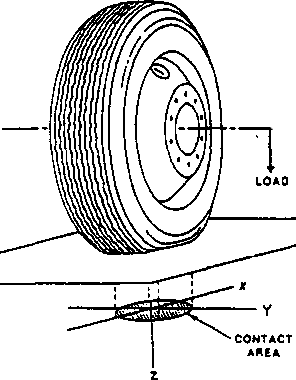
\includegraphics[width=0.2\textwidth]{../talk-dms/figs/tirecontact.png}

\vspace{-20mm}
\item pricing of American options
    \begin{itemize}
    \item[$\circ$] inequality-constrained Black-Scholes model
    \end{itemize}

\vspace{1.5mm}
\item the geometry of glaciers %\hfill $\longleftarrow$ \emph{more soon}

\vspace{1.5mm}
\item first-semester calculus:
    $$u = \mathop{\textnormal{argmin}}_{x\in[a,b]} f(x) \quad \implies \quad f'(u)(v-u) \ge 0 \quad \forall v \in[a,b]$$
\end{itemize}

\vspace{-5mm}
\begin{center}
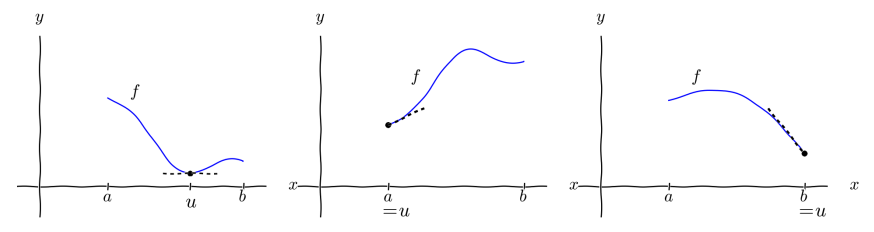
\includegraphics[height=25mm]{../talk-oxford/images/calcone.png}
\end{center}
\end{frame}


\AtBeginSection[]
{
  \begin{frame}{Outline}
    \tableofcontents[currentsection]
  \end{frame}
}

\section{nonlinear multigrid for PDEs}

\subsection{full approximation scheme (FAS)}

\begin{frame}{nonlinear 2-mesh scheme for PDEs}

\begin{center}
$\Omega^h$\, 
\includegraphics[height=0.16\textheight]{../talk-oxford/images/fine-grid.png} \hspace{25mm} 
\includegraphics[height=0.16\textheight]{../talk-oxford/images/coarse-grid.png} \,$\Omega^H$
\end{center}

\only<1>{
\begin{itemize}
\item consider a nonlinear elliptic PDE problem:
	$${\color{FireBrick} F(u) = \ell}$$

	\begin{itemize}
	\item[$\circ$] $\mathcal{V}=H^1(\Omega)$, $F : \mathcal{V} \to \mathcal{V}'$ continuous, $\ell\in \mathcal{V}'$
	\end{itemize}
\item discretization\footnote{discretization = finite element (FE) method, throughout this talk} gives algebraic system on fine mesh $\Omega^h$:
    $${\color{FireBrick} F^h(u^h) = \ell^h}$$
\item suppose $w^h$ is a not-yet-converged iterate:
    $$r^h=\ell^h - F^h(w^h), \qquad \|r^h\| > \text{TOL}$$
\end{itemize}
}
\only<2>{
\begin{itemize}
\item how can we improve $w^h$ \emph{without} globally linearizing $F^h$?

	\begin{itemize}
	\item are there alternatives to Newton's method?
	\end{itemize}
\item rewrite the equation as the nonlinear \emph{correction equation}
    $${\color{FireBrick} F^h(u^h) - F^h(w^h) = r^h}$$
\item \underline{for $F^h$ linear}, convert the correction eqn to the \emph{error equation}
    $$F^h(e^h) = r^h,$$
with approximate solution $\tilde e^h$, and update $w^h \leftarrow w^h+\tilde e^h$
\end{itemize}
}
\only<3>{
\begin{itemize}
\item there are fast \emph{smoothers}: inexpensive algorithms which improve $w^h$ by efficiently removing high-frequency error components
	\begin{itemize}
	\item sweeping through and solving nodewise problems (nonlinear Gauss-Seidel) is a smoother
	\end{itemize}
\item how about low-frequency error components?
\item \emph{idea}: use a coarser mesh $\Omega^H$ to estimate $u^h$ in the correction eqn
\end{itemize}

\vspace{5mm}
}
\only<4>{
\begin{itemize}
\item Brandt's (1977) \emph{full approximation scheme} (FAS) equation:
	$${\color{FireBrick} F^H(u^H) - F^H(\iR w^h) = R \, r^h(w^h)}$$

    \begin{itemize}
    \item[$\circ$] $\iR:\mathcal{V}^h \to \mathcal{V}^H$ is node-wise \emph{injection}
    \item[$\circ$] $R:(\mathcal{V}^h)' \to (\mathcal{V}^H)'$ is \emph{canonical restriction}
    \item[$\circ$] note: if $w^h=u^h$ exactly then $u^H = \iR w^h$ since $F^H$ injective
    \end{itemize}

\item let $\ell^H = F^H(\iR w^h) + R\, r^h(w^h)$
\item rewritten FAS equation:
    $${\color{FireBrick} F^H(u^H) = \ell^H}$$
\end{itemize}
}
\end{frame}


\begin{frame}{full approximation scheme (FAS): 2-mesh cycle}

\begin{center}
fine mesh $=\Omega^h$\, 
\includegraphics[height=0.14\textheight]{../talk-oxford/images/fine-grid.png} \hspace{15mm} 
\includegraphics[height=0.14\textheight]{../talk-oxford/images/coarse-grid.png} \,$\Omega^H=$ coarse mesh
\end{center}

\begin{align*}
&\text{pre-smooth over fine:} & & \text{smoother on } w^h \\
&\text{restrict:}                   & &\ell^H = F^H(\iR w^h) + R\, r^h(w^h) \\
&\text{coarse solve:}               & &F^H(w^H) = \ell^H \\
&\text{correct:}                    & &w^h \leftarrow w^h + P(w^H - \iR w^h) \\
&\text{post-smooth over fine:} & & \text{smoother on } w^h
\end{align*}

\bigskip
{\small
\begin{itemize}
\item $R: (\mathcal{V}^h)' \to (\mathcal{V}^H)'$ is \emph{canonical restriction}
\item $P: \mathcal{V}^H \to \mathcal{V}^h$ is \emph{canonical prolongation}
\item $\iR: \mathcal{V}^h \to \mathcal{V}^H$ is \emph{injection}
\item (restrict$+$coarse solve$+$correct) \, $=$ \, \emph{FAS coarse grid correction}
\end{itemize}
}
\end{frame}


\begin{frame}{nonlinear multigrid by FAS: \only<1>{V-cycle}\only<2>{FMG cycle}}

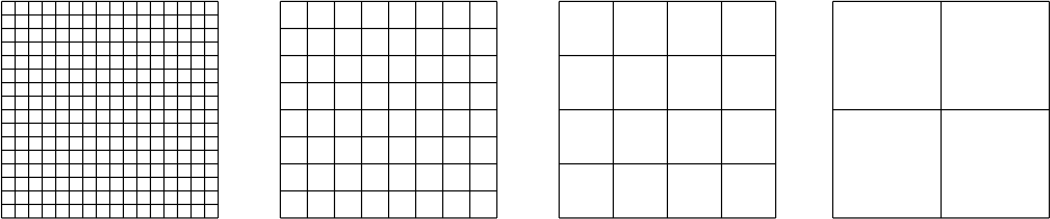
\includegraphics[height=0.2\textheight]{../talk-oxford/images/mg-grids.png}

\hspace{4mm} $J=3$ \hspace{13mm} $j=2$ \hspace{13mm} $j=1$ \hspace{12mm} $j=0$

\bigskip
\only<1>{
\begin{columns}
\begin{column}{0.75\textwidth}
{\small
\begin{pseudo}
\pr{fas-vcycle}$(\ell^J;w^J)$: \\+
    for $j=J$ downto $j=1$ \\+
      $\text{\pr{smooth}}^{\text{\id{down}}}(\ell^j; w^j)$ \\
      $w^{j-1} = \iR w^j$ \\
      $\ell^{j-1} = F^{j-1}(w^{j-1}) + R \left(\ell^j - F^j(w^j)\right)$ \\-
    $\text{\pr{solve}}(\ell^0;w^0)$ \\
    for $j=1$ to $j=J$ \\+
      $w^j \gets w^j + P (w^{j-1} - \iR w^j)$ \\
      $\text{\pr{smooth}}^{\text{\id{up}}}(\ell^j;w^j)$ \\-
\end{pseudo}
}
\end{column}
\begin{column}{0.25\textwidth}
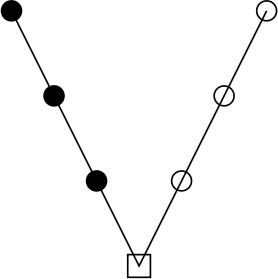
\includegraphics[width=0.7\textwidth]{../talk-oxford/images/mg-vcycle.png}
\end{column}
\end{columns}
}
\only<2>{
\vspace{6mm}

\centering
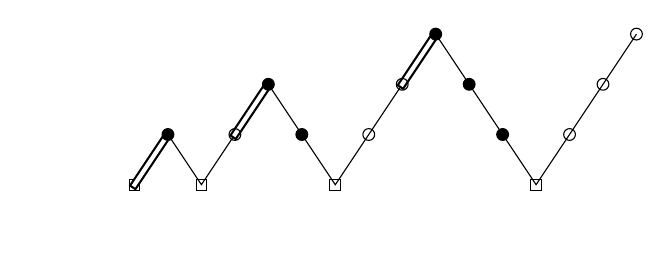
\begin{tikzpicture}[scale=0.85]
  \pgfmathsetmacro\hstep{0.5}
  \pgfmathsetmacro\vstep{0.75}
  \pgfmathsetmacro\ceps{0.08}   % size of square for coarse grid

% initial restriction to coarsest
  \pgfmathsetmacro\hoff{0*\hstep}
  %\draw[shift={(\hoff,0)},gray,line width=1.0mm] (0.0,3*\vstep) -- (\hstep,2*\vstep) --  (2*\hstep,\vstep) -- (3*\hstep,0.0);
  \draw[shift={(\hoff,0)}]     (3*\hstep-\ceps,-\ceps) rectangle (3*\hstep+\ceps,+\ceps);
  \draw[shift={(\hoff,0)},black,thick,double,double distance between line centers=0.8mm,line cap=rect] (3*\hstep,0.0) -- (4*\hstep,\vstep);

% V-cycle to level 1
  \pgfmathsetmacro\hoff{4*\hstep}
  \draw[shift={(\hoff,0)},black,thin] (0.0,\vstep) -- (\hstep,0.0) -- (2*\hstep,\vstep);
  \draw[shift={(\hoff,0)},black,thick,double,double distance between line centers=0.8mm,line cap=rect] (2*\hstep,\vstep) -- (3*\hstep,2*\vstep);
  \filldraw[shift={(\hoff,0)}] (0.0,\vstep) circle (2.5pt);
  \draw[shift={(\hoff,0)}]     (\hstep-\ceps,-\ceps) rectangle (\hstep+\ceps,+\ceps);
  \draw[shift={(\hoff,0)}]     (2*\hstep,\vstep) circle (2.5pt);

% V-cycle to level 2
  \pgfmathsetmacro\hoff{7*\hstep}
  \draw[shift={(\hoff,0)},black,thin] (0.0,2*\vstep) --  (\hstep,\vstep) -- (2*\hstep,0.0) -- (3*\hstep,\vstep) -- (4*\hstep,2*\vstep);
  \draw[shift={(\hoff,0)},black,thick,double,double distance between line centers=0.8mm,line cap=rect] (4*\hstep,2*\vstep) -- (5*\hstep,3*\vstep);
  \filldraw[shift={(\hoff,0)}] (0.0,2*\vstep) circle (2.5pt);
  \filldraw[shift={(\hoff,0)}] (\hstep,\vstep) circle (2.5pt);
  \draw[shift={(\hoff,0)}]     (2*\hstep-\ceps,-\ceps) rectangle (2*\hstep+\ceps,+\ceps);
  \draw[shift={(\hoff,0)}]     (3*\hstep,\vstep) circle (2.5pt);
  \draw[shift={(\hoff,0)}]     (4*\hstep,2*\vstep) circle (2.5pt);

% V-cycle to finest (level 3)
  \pgfmathsetmacro\hoff{12*\hstep}
  \draw[shift={(\hoff,0)},black,thin] (0.0,3*\vstep) -- (\hstep,2*\vstep) --  (2*\hstep,\vstep) -- (3*\hstep,0.0) -- (4*\hstep,\vstep) -- (5*\hstep,2*\vstep) -- (6*\hstep,3*\vstep);
  \filldraw[shift={(\hoff,0)}] (0.0,3*\vstep) circle (2.5pt);
  \filldraw[shift={(\hoff,0)}] (\hstep,2*\vstep) circle (2.5pt);
  \filldraw[shift={(\hoff,0)}] (2*\hstep,\vstep) circle (2.5pt);
  \draw[shift={(\hoff,0)}]     (3*\hstep-\ceps,-\ceps) rectangle (3*\hstep+\ceps,+\ceps);
  \draw[shift={(\hoff,0)}]     (4*\hstep,\vstep) circle (2.5pt);
  \draw[shift={(\hoff,0)}]     (5*\hstep,2*\vstep) circle (2.5pt);
  \draw[shift={(\hoff,0)}]     (6*\hstep,3*\vstep) circle (2.5pt);

  \draw[white] (0, -\vstep) circle (2.5pt);
\end{tikzpicture}



FMG $=$ full multigrid

\vspace{6mm}
}
\end{frame}


\begin{frame}{FAS reputation}

\begin{itemize}
\item FAS multigrid is a \emph{fast solver} on nice nonlinear PDE problems
    \begin{itemize}
    \item[$\circ$] example: Liouville-Bratu equation $-\nabla^2 u - e^u = 0$
    \end{itemize}

\bigskip
\item<2> what does ``fast solver'' mean?
\end{itemize}

\begin{block}<2>{definition} a solver is \emph{optimal} if work is $O(N)$ for $N$ unknowns
\end{block}

\begin{itemize}
\item<2> one can measure work in flops or run-time
\item<2> constant iterations of $O(N)$ method $\implies$ optimal
\end{itemize}
\end{frame}


\section{FASCD = FAS multigrid for VIs using constraint decomposition}

\subsection{results on test problems}

\begin{frame}{test problem 1: classical obstacle problem}

\only<1>{recall:

\centerline{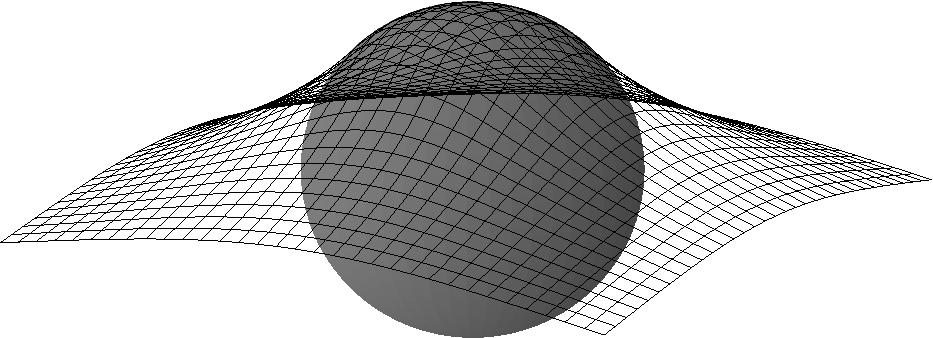
\includegraphics[width=0.9\textwidth]{../talk-oxford/images/obstacle65.pdf}}}
\only<2>{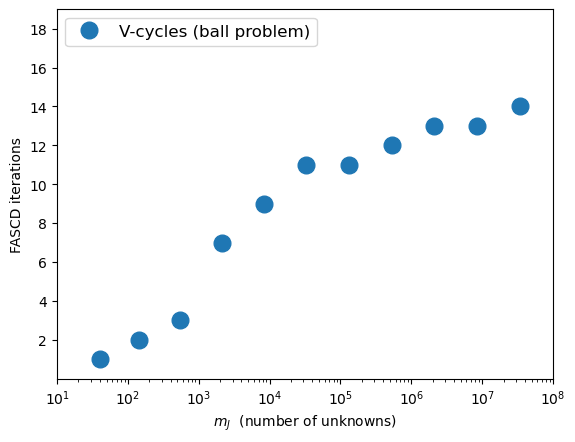
\includegraphics[width=0.75\textwidth]{figs/ballitersV.png}}\only<3>{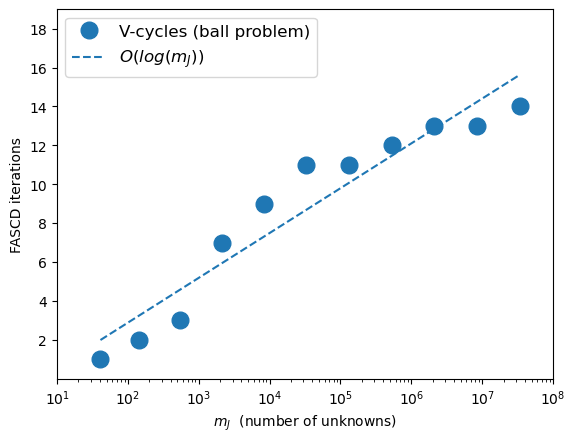
\includegraphics[width=0.75\textwidth]{figs/ballitersVlog.png}}\only<4>{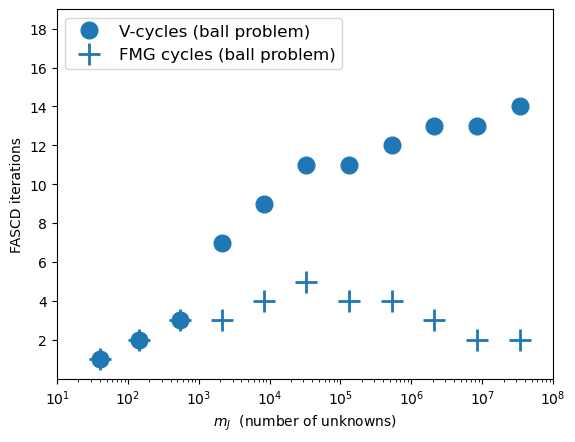
\includegraphics[width=0.75\textwidth]{figs/ballitersVF.png}}\only<5>{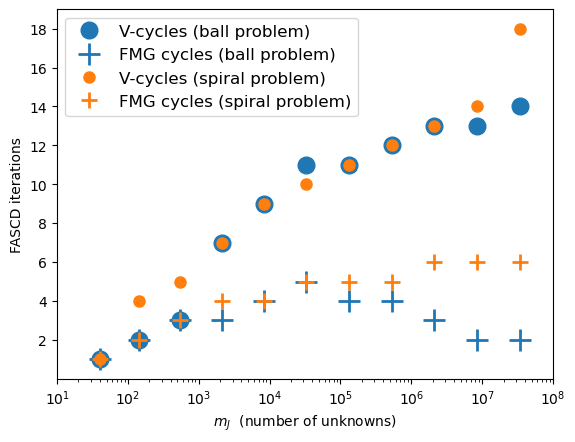
\includegraphics[width=0.75\textwidth]{figs/bothitersVF.png}} \hfill
\only<2-4>{
\includegraphics[width=0.2\textwidth]{../paper/fixfigs/ball-set.png}}%
\only<5>{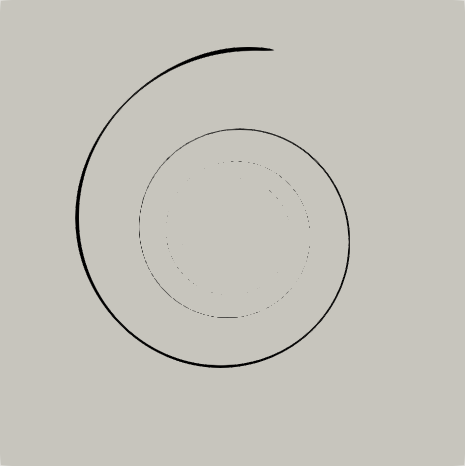
\includegraphics[width=0.2\textwidth]{../paper/fixfigs/spiral-set.png}}

\only<2-5>{\noindent \scriptsize
\emph{all results from Bueler \& Farrell (2024)}}
\end{frame}


\begin{frame}{test problem 2: advection-diffusion}

\begin{itemize}
\item $u(x)$ is a concentration in $\Omega \subset \RR^d$: \qquad $\boxed{0\le u\le 1}$
\item concentration evolves by diffusion, advection, and source:
    $$-\eps \grad^2 u + \bm{X}\cdot \grad u = \sigma$$
\item two active sets:
    $$\underline{A}_u = \{u(x) = 0\} \hspace{22mm} \overline{A}_u = \{u(x) = 1\} \hspace{8mm}$$
\end{itemize}

\centering

\includegraphics[width=0.27\textwidth]{../paper/fixfigs/poll2d-zero-set.png} \hspace{18mm}
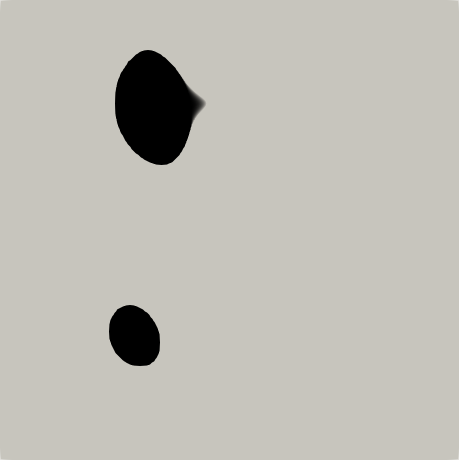
\includegraphics[width=0.27\textwidth]{../paper/fixfigs/poll2d-one-set.png}
\end{frame}


\begin{frame}{test problem 2: advection-diffusion}

\begin{center}
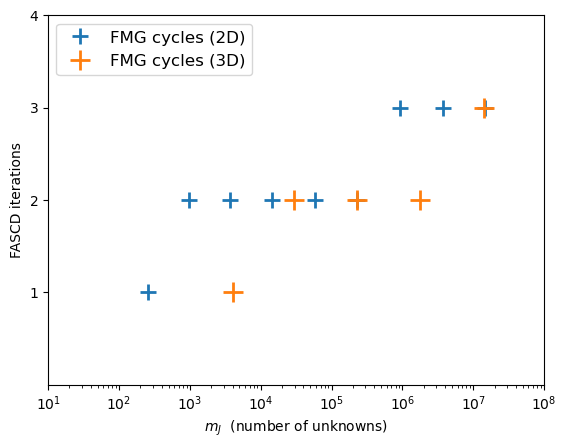
\includegraphics[width=0.75\textwidth]{figs/advdiff.png}
\end{center}

\vspace{-3mm}
\hfill \tiny \emph{Bueler \& Farrell (2024)}
\end{frame}


\subsection{an application}

\begin{frame}{``where are the glaciers?'' is a free-boundary problem}

\bigskip
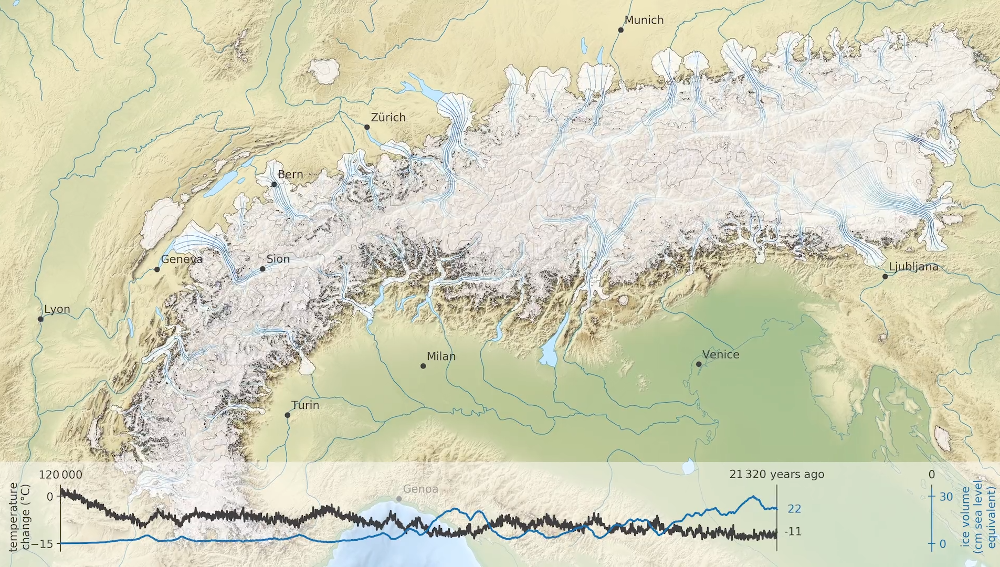
\includegraphics[width=1.01\textwidth]{../talk-oxford/images/alps-seguinot2018.png}

\vspace{-2mm}
\hfill {\tiny \emph{Seguinot et al.~(2018)}}
\end{frame}


\begin{frame}{the glacier free-boundary problem}

\begin{itemize}
\item a \emph{glacier} is an incompressible, viscous fluid driven by gravity, with mass from a climate which adds or removes ice at a signed rate, over a fixed bed topography with elevation $b$
\item to find: ice surface elevation $s$ (and velocity $\bu$) subject to constraint $\boxed{s\ge b}$
\item test case: ice sheet the size of Greenland

\bigskip
\begin{center}
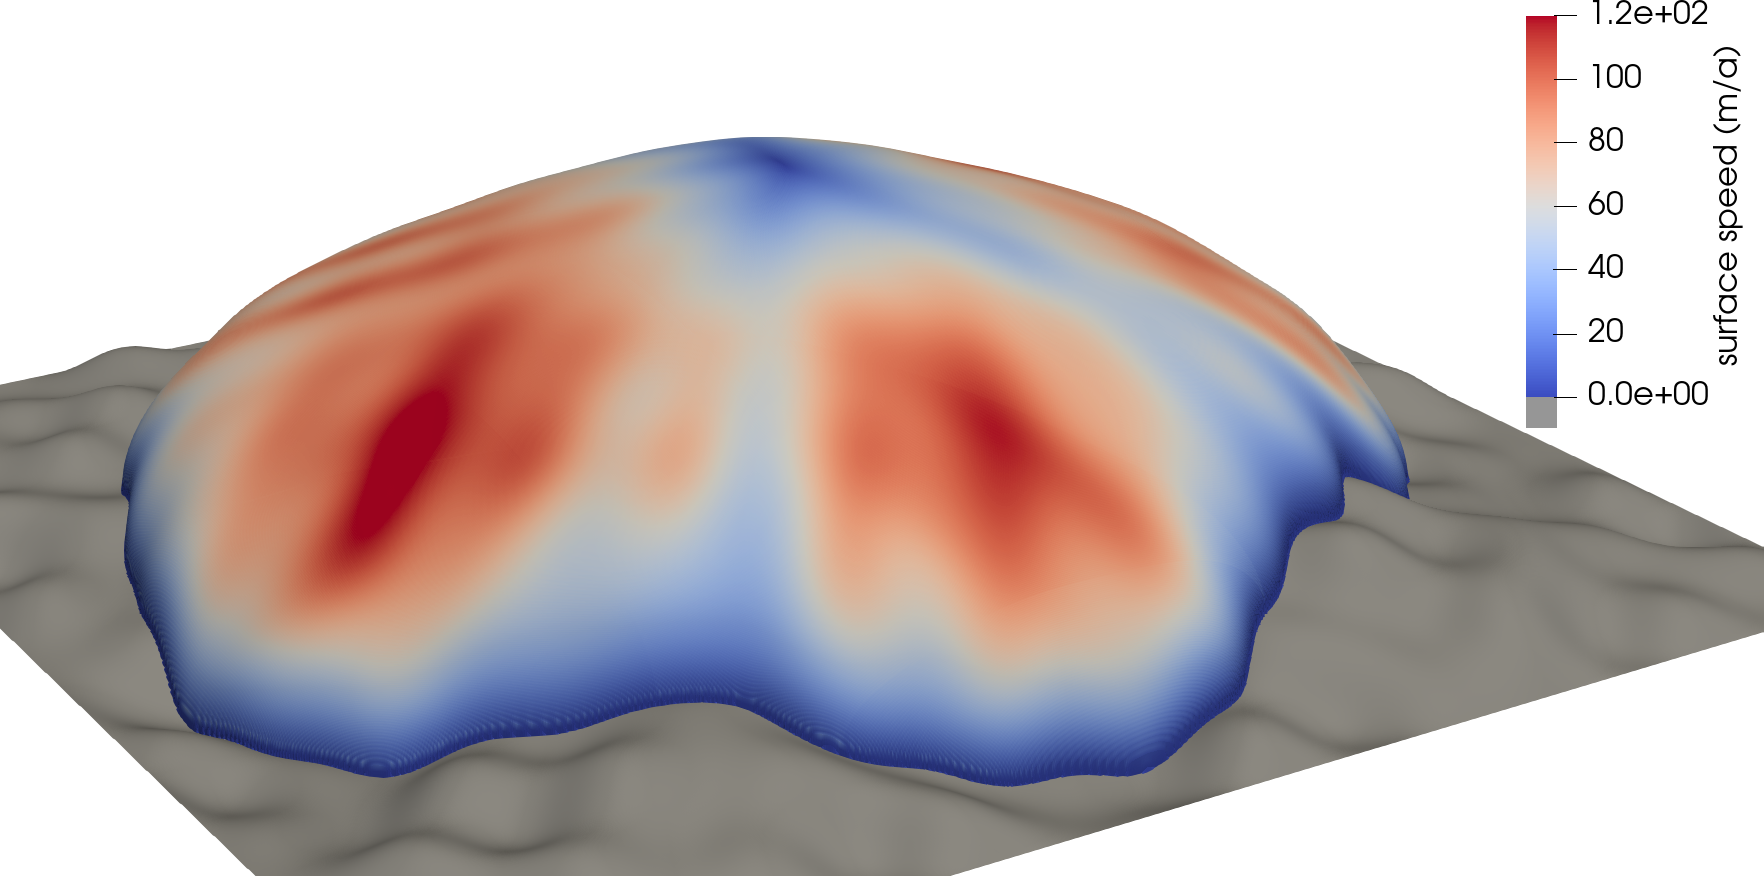
\includegraphics[width=0.65\textwidth]{../paper/fixfigs/sialev8scene.png}
\end{center}
\end{itemize}
\end{frame}


\begin{frame}{glacier free-boundary problem: steady VI form}

\begin{itemize}
\item admissible surface elevations:
    $$\mathcal{K} = \left\{r \in \mathcal{V} \,:\, r \ge b\right\}$$
\item steady-state VI problem for surface elevation $s\in\mathcal{K}$:
       $$\ip{\Phi(s) - a}{r-s} \ge 0 \quad \text{ for all } r \in \mathcal{K}$$
where $\Phi(s)=- \bu|_s \cdot \bn_s$
\item in the isothermal, nonsliding, \emph{shallow ice approximation}\footnote{$=$ \emph{a highly-simplified view of conservation of momentum, in which} $(s-b)^{8/3} \in W^{1,4}(\Omega)$ \emph{so} $\mathcal{V} \stackrel{?}{=} (W^{1,4})^{3/8}$ \hfill \emph{Jouvet \& Bueler (2012)}} case:
\begin{align*}
\Phi(s) &= - \bu|_s \cdot \bn_s \\
        &= - \frac{\gamma}{4} (s-b)^{4} |\grad s|^{4} - \grad \cdot\left(\frac{\gamma}{5} (s-b)^{5} |\grad s|^{2} \grad s\right)
\end{align*}
\end{itemize}
\end{frame}


\begin{frame}{optimality and weak scaling on a glacier problem}

\begin{itemize}
\item optimality of FMG solver (left)
\item good parallel \emph{weak scaling} (right)
    \begin{itemize}
    \item[$\circ$] each processor owns $641\times 641$ (sub) mesh
    \item[$\circ$] $P=1024$ run had $20481^2=4.1\times 10^8$ unknowns and 88 meter resolution
    \end{itemize}
\end{itemize}

\bigskip
\mbox{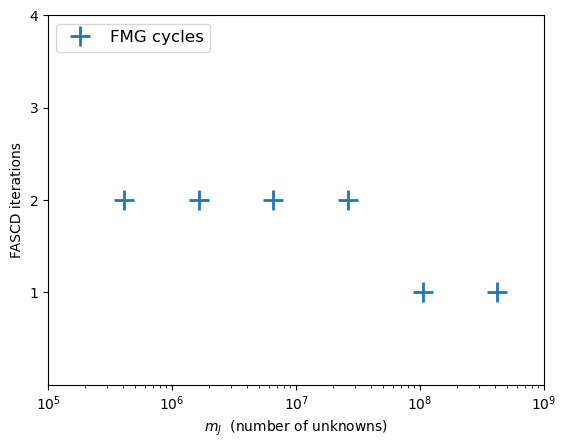
\includegraphics[width=0.5\textwidth]{figs/sia.png} 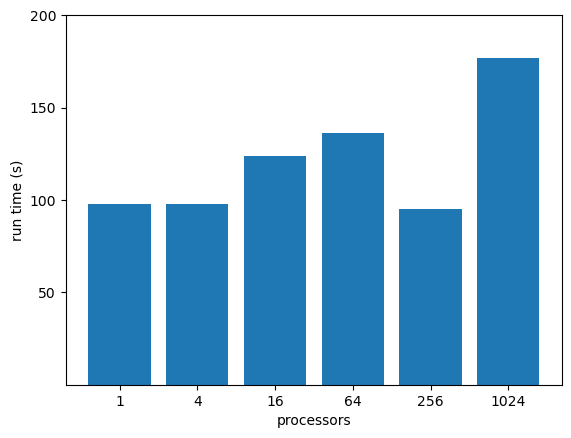
\includegraphics[width=0.5\textwidth]{../talk-dms/figs/siaweaktime.png}}

\hfill \scriptsize
\emph{Bueler \& Farrell (2024)}
\end{frame}


\subsection{the algorithm}

\begin{frame}{an FAS multigrid strategy for VIs}

\begin{itemize}
\item new algorithm:\footnote{E.~Bueler \& P.~Farrell (2024). \emph{A full approximation scheme multilevel method for nonlinear variational inequalities}, SIAM J.~Sci.~Comput.~46 (4) \sdoi{10.1137/23M1594200}}

\bigskip
{\color{FireBrick} FASCD = full approximation scheme constraint decomposition}

\bigskip
\item<2> but what is ``constraint decomposition''?
\end{itemize}
\end{frame}


\begin{frame}{subspace decomposition}

\hfill 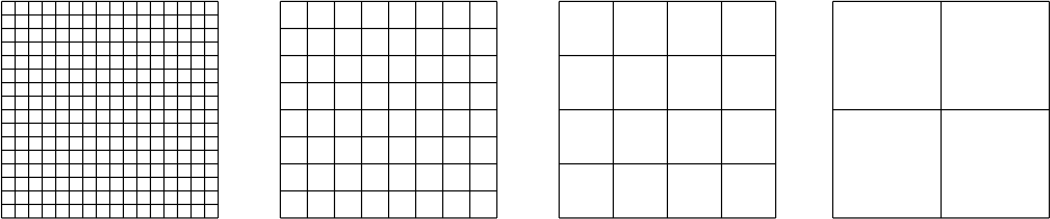
\includegraphics[height=0.12\textheight]{../talk-oxford/images/mg-grids.png}

{\footnotesize
\hfill $\Omega^3$ \hspace{8.5mm} $\Omega^2$ \hspace{8.5mm} $\Omega^1$ \hspace{8.5mm} $\Omega^0$ \hspace{1mm}
}

\begin{itemize}
\item start with nested meshes:
    $$\Omega^j \subset \Omega^{j+1}$$
\item the FE vector spaces $\mathcal{V}^j$ over $\Omega^j$ are also nested:
    $$\mathcal{V}^j \subset \mathcal{V}^{j+1}$$
\item $\mathcal{V}^J = \sum_{i=0}^J \mathcal{V}^i$ is called a \emph{subspace decomposition}

    \begin{itemize}
    \item[$\circ$] \emph{non}-unique vector space sum
    %\item[$\circ$] one may analyze linear multigrid for PDEs via subspace decomposition
    \end{itemize}
\end{itemize}
\end{frame}


\begin{frame}{constraint decomposition}

\begin{itemize}
\item Tai (2003): constraint decomposition \emph{non-trivially} extends subspace decomposition to convex subsets
\item suppose $\mathcal{K}^J \subset \mathcal{V}^J$ is a closed and convex subset
\item suppose $\mathcal{V}^J = \sum_{i=0}^J \mathcal{V}^i$ is a subspace decomposition
\begin{block}{definition}
$\ds \mathcal{K}^J = \sum_{i=0}^J \mathcal{K}^i$ \quad is a \emph{constraint decomposition} (CD) if there are closed and convex subsets $\mathcal{K}^i\subset \mathcal{V}^i$, and (nonlinear) projections $\Pi_i : \mathcal{K}^J \to \mathcal{K}^i$, so that $\ds v = \sum_{i=0}^J \Pi_i v$ and a stability condition applies (not shown)
\end{block}
\end{itemize}
\end{frame}


\begin{frame}{constraint decomposition}

\begin{itemize}
\item observation: generally $\mathcal{K}^i \not\subset \mathcal{K}^J$
\end{itemize}

\bigskip
\begin{center}
\includegraphics[width=0.6\textwidth]{../paper/genfigs/cartoon.pdf}

\medskip
{\small obstacle problem on a two-point mesh with $\mathcal{V} \cong \RR^2$}
\end{center}
\end{frame}


\begin{frame}{iterations over a constraint decomposition}

\begin{itemize}
\item Tai proposed abstract iterations for solving $VI(F,\ell,\mathcal{K})$ over a CD
\item specifically the multiplicative/serial iteration:

{\small
\begin{pseudo}[left-margin=-5mm]
\pr{cd-mult}(u)\text{:} \\+
    for $i = 0,\dots,m-1$: \\+
        find $w_i\in \cK_i$ s.t. \\+
            $\displaystyle \Big<F\Big(\sum_{j<i} w_j + w_i + \sum_{j>i} \Pi_j u\Big),\, v_i - w_i\Big> \ge \ip{\ell}{v_i - w_i} \,\forall v_i \in \cK_i$ \\--
    return $w=\sum_i w_i\in\cK$
\end{pseudo}
}

\item \dots but not practical because you evaluate residuals on finest level
\item two techniques make a practical solver (Bueler \& Farrell, 2024):

    \begin{itemize}
    \item[$\circ$] \emph{defect obstacles} on each level  \hfill {\scriptsize Gr\"aser \& Kornhuber (2009)}
    \item[$\circ$] \emph{FAS coarse corrections}  \hfill {\scriptsize Brandt (1977)}
    \end{itemize}
\end{itemize}
\end{frame}


\begin{frame}{defect obstacles}

\begin{itemize}
\item suppose $\mathcal{K} = \{v \ge \psi\}$ in an obstacle problem
\begin{block}{definition}
for finest-level admissible set $\mathcal{K}^J = \{v^J\ge \psi^J\} \subset \mathcal{V}^J$ and an iterate $w^J \in \mathcal{K}^J$, the \emph{defect obstacle} is
    $$\chi^J = \psi^J - w^J \in \mathcal{V}^J$$
\end{block}

    \begin{itemize}
    \item[$\circ$] note $\chi^J \le 0$
    \end{itemize}
\item generate the CD through

defect obstacles $\chi^j$ on each

level via \emph{monotone restriction}:

$$\chi^j = R^{\oplus} \chi^{j+1} \phantom{smdlfkaj asdfklj asdf sdfaa asddfas dsa}$$

    \begin{itemize}
    \item[$\circ$] a \emph{nonlinear} operator
    \end{itemize}
\end{itemize}

\vspace{-25mm}
\hfill \mbox{\definecolor{seabornblue}{rgb}{0.2980392156862745, 0.4470588235294118, 0.6901960784313725}
\definecolor{seaborngreen}{rgb}{0.3333333333333333, 0.6588235294117647, 0.40784313725490196}
\definecolor{seabornred}{rgb}{0.7686274509803922, 0.3058823529411765, 0.3215686274509804}

\begin{tikzpicture}[scale=1.0]
  \foreach \k in {0, 1, 2, 3, 4} {
    %\filldraw[seabornblue, fill=seabornblue] ({cos(deg(2*\k*pi/5))}, {sin(deg(2*\k*pi/5))}) circle (1.5pt);
    \node (A) at ({0.5*cos(deg(2*\k*pi/5)) + 0.5*cos(deg(2*(\k+1)*pi/5))}, {0.5*sin(deg(2*\k*pi/5)) + 0.5*sin(deg(2*(\k+1)*pi/5))}) {};
    \node (B) at ({0.5*cos(deg(2*\k*pi/5))}, {0.5*sin(deg(2*\k*pi/5))}) {};
    \node (C) at ({0.5*cos(deg(2*(\k+1)*pi/5))}, {0.5*sin(deg(2*(\k+1)*pi/5))}) {};
    \node (D) at ({cos(deg(2*\k*pi/5))}, {sin(deg(2*\k*pi/5))}) {};
    \node (E) at ({cos(deg(2*(\k+1)*pi/5))}, {sin(deg(2*(\k+1)*pi/5))}) {};

    \draw [-,gray, very thick] (A.center) -- (B.center);
    \draw [-,gray, very thick] (B.center) -- (C.center);
    \draw [-,gray, very thick] (C.center) -- (A.center);

    \draw [black, ultra thick] (0, 0) -- (D.center);
    \draw [black, ultra thick] (D.center) -- (E.center);

    \filldraw[seaborngreen] (A) circle (1.5pt);
    \filldraw[seaborngreen] (B) circle (1.5pt);
    \filldraw[seaborngreen] (C) circle (1.5pt);
    \filldraw[seaborngreen] (D) circle (1.5pt);
    \filldraw[seaborngreen] (E) circle (1.5pt);

  }
  \filldraw[seabornblue] (0, 0) circle (2.5pt);
  
  \filldraw[seabornblue] (2.5, 0.5) circle (2.5pt);
  \node at (5.0, 0.5) {$= \text{coarse mesh node}$};
  \filldraw[seaborngreen] (2.5, 0.0) circle (1.5pt);
  \node (fine) at (4.5, 0.0) {$= \text{fine mesh node}$};
\end{tikzpicture}
}
\end{frame}


\begin{frame}{up and down CDs in FASCD}

\begin{center}
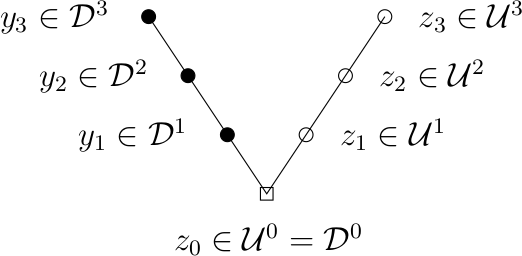
\includegraphics[width=0.4\textwidth]{../talk-oxford/images/fascd-vcycle.png}
\end{center}

\begin{itemize}
\item upward direction in V-cycle uses larger admissible sets:
    $$\mathcal{U}^j = \{z^j \ge \chi^j\}$$
\item downward sets are smaller to guarantee admissibility of the upcoming coarse correction:
    $$\mathcal{D}^j = \{y^j \ge \phi^j=\chi^j - \chi^{j-1}\}$$
\item $\ds \mathcal{U}^j = \sum_{i=0}^j \mathcal{D}^i$ is a CD of the $j$th-level admissible set
\end{itemize}
\end{frame}


\begin{frame}{up and down CDs in FASCD}

\begin{center}
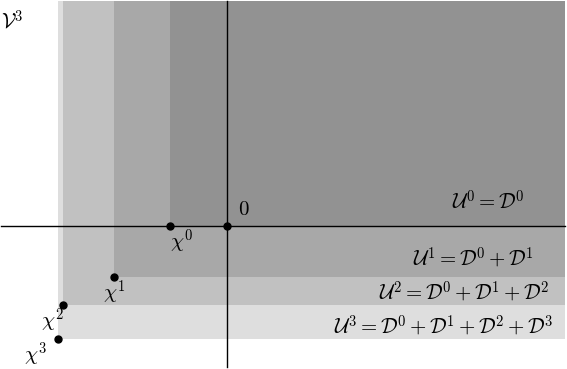
\includegraphics[width=0.7\textwidth]{../talk-dms/figs/innerconeapprox.png}
\end{center}

\begin{itemize}
\item all sets $\mathcal{U}^j$ and $\mathcal{D}^j$ include the origin
\end{itemize}
\end{frame}


\begin{frame}{FASCD = full approximation scheme constraint decomposition}

\vspace{-2mm}
\begin{pseudo}[font=\small]
\pr{fascd-vcycle}(J,\ell^J,\psi^J;w^J)\text{:} \\+
    $\chi^J = \psi^J - w^J$ \\
    for $j=J$ downto $j=1$ \\+
      $\chi^{j-1} = \maxR \chi^j$ \\
      $\phi^j = \chi^j - P\chi^{j-1}$ \\
      $y^j = 0$ \\
      $\text{\pr{smooth}}^{\text{\id{down}}}(\ell^j,\phi^j,w^j;y^j)$ \\
      $w^{j-1} = \iR(w^j + y^j)$ \\
      $\ell^{j-1} = f^{j-1}(w^{j-1}) + R \left(\ell^j - f^j(w^j+y^j)\right)$ \\-
    $z^0 = 0$ \\
    $\text{\pr{solve}}(\ell^0,\chi^0,w^0;z^0)$  \\
    for $j=1$ to $j=J$ \\+
      $z^j = y^{j} + P z^{j-1}$ \\
      $\text{\pr{smooth}}^{\text{\id{up}}}(\ell^j,\chi^j,w^j;z^j)$  \\-
    return $w^J+z^J$
\end{pseudo}

\vspace{-2mm}
\tiny
\begin{itemize}
\item[] \emph{(unilateral (lower obstacle only) version shown for simplicity)}
\end{itemize}
\end{frame}


\begin{frame}{V-cycle: visualization on a 1D problem}

\centering
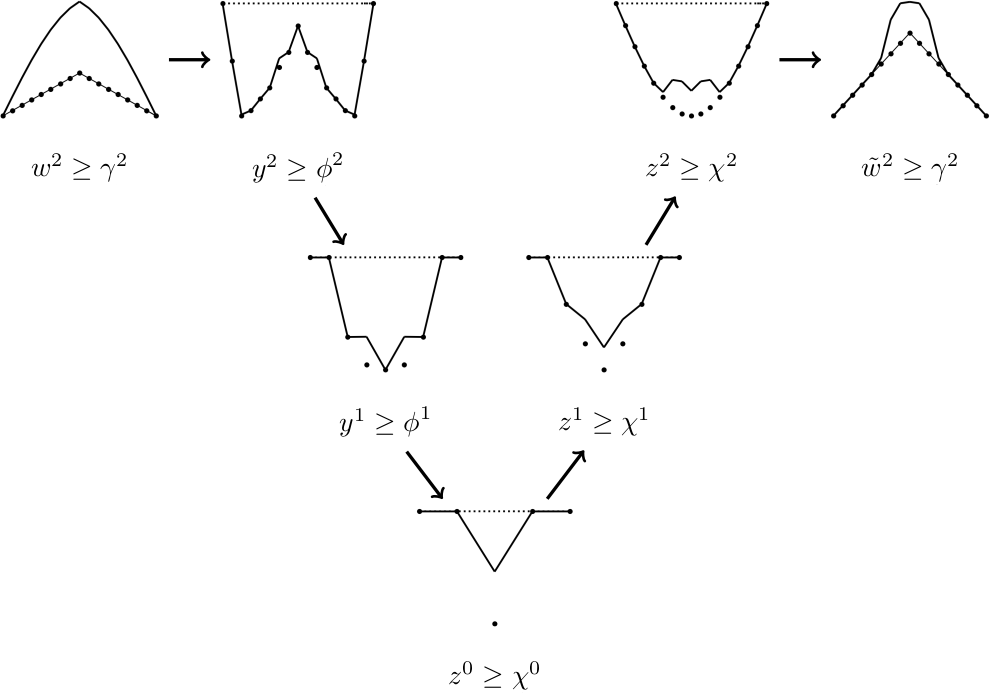
\includegraphics[width=0.85\textwidth]{../talk-dms/figs/vcycle-visualized.png}
\end{frame}


\begin{frame}{specifics}

see Bueler \& Farrell (2024) for:
\begin{itemize}
\item generalization to upper and lower obstacles:
    $$\mathcal{K}^J = \{\underline{\psi}^J \le v^J \le \overline{\psi}^J\}$$
\item stopping criteria
    \begin{itemize}
    \item[$\circ$] evaluates CP/KKT conditions
    \end{itemize}
\item FMG cycle
\item details of the $O(m_j)$ smoother used in the results: a few iterations of projected, reduced-space Newton with a few iterations of CG+ICC or GMRES+ILU on the linear step equations
\end{itemize}
\end{frame}


\begin{frame}{summary and outlook}

\begin{itemize}
\item FASCD = new multilevel solver for VI (free-boundary) problems
    \begin{itemize}
    \item[$\circ$] implemented in Python using the Firedrake library
    \item[$\circ$] observed optimality, and actually fast on tested problems
    \end{itemize}
\item many things \textbf{{\color{FireBrick} to do}}:
    \begin{itemize}
    \item[$\circ$] implement in C within PETSc
    \item[$\circ$] prove convergence; compare (Reusken, 1988)
    \item[$\circ$] mesh adaptivity, better smoothers, parabolic examples, \dots
    \end{itemize}
\end{itemize}

\bigskip\bigskip
\begin{minipage}[T]{0.25\textwidth}
\vspace{0pt}


\includegraphics[width=0.8\textwidth]{figs/QRbuelerfarrell.png}

\scriptsize paper in

SIAM J.~Sci.~Comput.
\end{minipage}
\hfill
\begin{minipage}[T]{0.25\textwidth}
\vspace{0pt}

\hfill 
\includegraphics[width=0.8\textwidth]{figs/QRfascd.png}

\scriptsize \hfill code at bitbucket

\phantom{foo}
\end{minipage}
\end{frame}


\begin{frame}{references}

{\footnotesize
% inputed at end of slides.tex

\newcommand{\sdoi}[1]{\,{\tiny \href{https://doi.org/#1}{doi:#1}}}
\begin{itemize}
\item A.~Brandt \& C.~Cryer (1983). \emph{Multigrid algorithms for the solution of linear complementarity problems \dots}, SIAM J.~Sci.~Stat.~Comput.~4 (4), 655--684 \sdoi{10.1137/0904046}
%FTITLE Multigrid algorithms for the solution of linear complementarity problems arising from free boundary problems
\item P.~Brune, M.~Knepley, B.~Smith, \& X.~Tu (2015). \emph{Composing scalable nonlinear algebraic solvers}, SIAM Review~57 (4), 535--565 \sdoi{10.1137/130936725}
\item E.~Bueler (2021). \emph{Conservation laws for free-boundary fluid layers}, SIAM J.~Appl.~Math.~81 (5), 2007--2032 \sdoi{10.1137/20M135217X}
%\item E.~Bueler (2022). \emph{Performance analysis of high-resolution ice-sheet simulations}, J.~Glaciol., \sdoi{10.1017/jog.2022.113}
\item G.~de Diego, P.~Farrell, \& I.~Hewitt (2022). \emph{Numerical approximation of viscous contact problems applied to glacial sliding}, J.~Fluid Mech.~938 (A21). \sdoi{10.1017/jfm.2022.178}
\item P.~Farrell, M.~Croci, \& T.~Surowiec (2020). \emph{Deflation for semismooth equations}, Optimization Methods \& Software 35 (6), 1248--1271 \sdoi{10.1080/10556788.2019.1613655}
\item C.~Gr{\"a}ser \& R.~Kornhuber (2009). \emph{Multigrid methods for obstacle problems}, J.~Comput.~Math., 1--44
\item T.~Isaac, G.~Stadler, \& O.~Ghattas (2015). \emph{Solution of nonlinear Stokes equations \dots ice sheet dynamics}, SIAM J.~Sci.~Comput., 37 (6), B804--B833 \sdoi{10.1137/140974407}
%FTITLE Solution of nonlinear Stokes equations discretized by high-order finite elements on nonconforming and anisotropic meshes, with application to ice sheet dynamics
\item G.~Jouvet \& E.~Bueler (2012). \emph{Steady, shallow ice sheets as obstacle problems \dots}, SIAM J.~Appl.~Math.~72 (4), 1292--1314 \sdoi{10.1137/110856654}
%FTITLE Steady, shallow ice sheets as obstacle problems: well-posedness and finite element approximation
\item G.~Jouvet \& J.~Rappaz (2011). \emph{Analysis and finite element approximation of a nonlinear stationary {S}tokes problem \dots}, Adv.~Numer.~Analysis 2011 (164581) \sdoi{10.1155/2011/164581}
%FTITLE Analysis and finite element approximation of a nonlinear stationary {S}tokes problem arising in glaciology
\item R.~Kornhuber (1994). \emph{Monotone multigrid methods for elliptic variational inequalities I}, Numer.~Math.~69, 167--184 \sdoi{10.1007/BF03325426}
\item A.~Reusken (1987). \emph{Convergence of the multigrid full approximation scheme \dots}, Numer.~Math.~52, 251--277 \sdoi{10.1007/BF01398879}
%FTITLE Convergence of the multigrid full approximation scheme for a class of elliptic mildly nonlinear boundary value problems
\item J.~Seguinot \& 5 others (2018).  \emph{Modelling last glacial cycle ice dynamics in the Alps}, The Cryosphere, 12 (10), 3265--3285 \sdoi{10.5194/tc-12-3265-2018}
%FAUTHORS Seguinot, J., Ivy-Ochs, S., Jouvet, G., Huss, M., Funk, M., & Preusser, F.
\item X.~Tai (2003). \emph{Rate of convergence for some constraint decomposition methods for nonlinear variational inequalities}, Numer.~Math.~93 (4), 755--786 \sdoi{10.1007/s002110200404}
\end{itemize}


}
\end{frame}

\end{document}
